%!tex root = ../main.tex

\section{Algorithm} \label{sec:algorithm}

In this section, we will introduce the basic idea of an essential algorithm that is used in the actual implementation discussed in section \ref{sec:implementation}.
The algorithm's purpose is to find a proof that a given LCL problem $\Pi$ is impossible to solve in PN model.
Here we specifically allow PN networks to have multiple edges.
Later we show that the unsolvability of a problem $\Pi$ in PN networks (with multiple edges) implies that it is also impossible to solve $\Pi$ in some simple PN networks.
%Thus it would be also impossible to solve using only simple PN networks.
%Given an LCL problem, the goal is to find a proof that it is impossible to solve the problem in PN model.

\begin{definition} \label{def:lcl_solvability}
    An LCL problem $\Pi$ is solvable in PN model if there exists a PN algorithm $A$ that can find a solution for $\Pi$ in all PN networks.
\end{definition}

\begin{theorem} \label{thm:lcl_nonsolvability}
    An LCL problem $\Pi$ is not solvable in PN model if there exists a PN network $N$ such that no PN algorithm $A$ can solve the $\Pi$ in $N$.
\end{theorem}
\begin{proof}
    Let us assume that the implication in the theorem is false (proof by contradiction).
    Thus $\exists N$ s.t. $\forall A$: $A$ cannot solve $\Pi$ in $N$.
    Also, the assumption states that $\Pi$ is solvable in PN model.
    This is in contradiction with Definition \ref{def:lcl_solvability}, since such network $N$ cannot exist when $P$ is solvable.
\end{proof}

As the Theorem \ref{thm:lcl_nonsolvability} hints, to show that a problem $\Pi$ is unsolvable, it is enough to find a counterexample, a PN network $N$ in which the problem $\Pi$ cannot be solved.

\begin{algorithm}
    \caption{Counterexample finder algorithm}
    \label{alg:test}
    \begin{algorithmic}[1] % The number tells where the line numbering should start
        \Procedure{Find}{$n_{low},n_{high}, \Pi$} \Comment{Graph bounds $n_{low}$ and $n_{high}$, LCL problem $\Pi$}
            %\State $r\gets a \bmod b$
            \For{$n\gets n_{low}, n_{high}$} \Comment{Iterate graph sizes from lowest to highest}
                \State $G_n \gets \operatorname{generate\_graphs}(n)$ \Comment{$G_n$ is a list of all graphs}
                \ForEach{$g \in G_n$}
                    \If {$\operatorname{is\_solvable}(\Pi, g)$}
                        \State \Return $g$
                    \EndIf
                \EndFor
            \EndFor\label{euclidendwhile}
            \State \Return \Comment{No counterexample found. Return nothing.}
        \EndProcedure
    \end{algorithmic}
\end{algorithm}

%TODO Continue from here and below. I believe that the algorithm above needs an explanation. Some implementation "details" from below should probably be moved to different section, maybe under 6. implementation. I do not know how much I should talk about SAT, maybe not at all.

%To prove this we first assume the opposite.
%That is, the problem $\Pi$ is possible to be solved in PN model.
%Then we try to find a counterexample that proves the assumption to be false.
%A graph in which we cannot find any viable labelling is a good counterexample, as this directly shows that we cannot solve the LCL problem in every graph.
%Therefore by finding a counterexample we show that the problem is impossible to be solved in PN model.

For each pair of LCL problem and graph, we want to be able to check if labelling is impossible.
To perform the checking, we first encode the problem and graph into a SAT problem.
Then we leverage the power of SAT solvers to solve the SAT problem.
We feed the SAT problem into the solver, which returns either SAT (satisfiable) or UNSAT (unsatisfiable) as a result.
In case the result is UNSAT, we have found a counterexample and we are done.
Otherwise we can continue searching using some other graph.
The routine is illustrated on Figure \ref{fig:implementatio:idea:1}.

\begin{figure}[H]
\centering
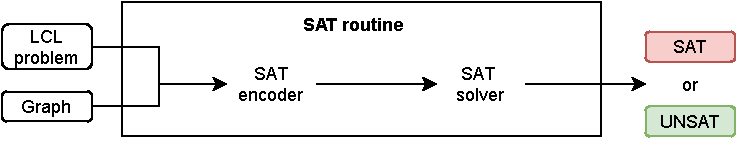
\includegraphics[]{diagrams/implementation_idea_diagram2.pdf}
\caption{The SAT routine. When given a graph and an LCL problem, it checks if a valid labelling exists.}
\label{fig:implementatio:idea:1}
\end{figure}

We repeat the routine for each graph in the current search space and terminate early if the result is UNSAT.
A solid and logical strategy is to first start with the smallest graphs and continue incrementally, increasing the size of graphs  after previous size has been searched entirely.
This can be indeed trivially automated as long as the routine is implemented.
User needs to only input the lower and upper bounds of graph sizes.
Here the graph size is the number of vertices, that is, $n=|V|$.
A search space can be for example every graph from $1$ to $15$.
Then the set of graphs would be $\{(V, E) : |V| \in \{1, 2, ..., 15\} \}$.

\begin{figure}[H]
\centering
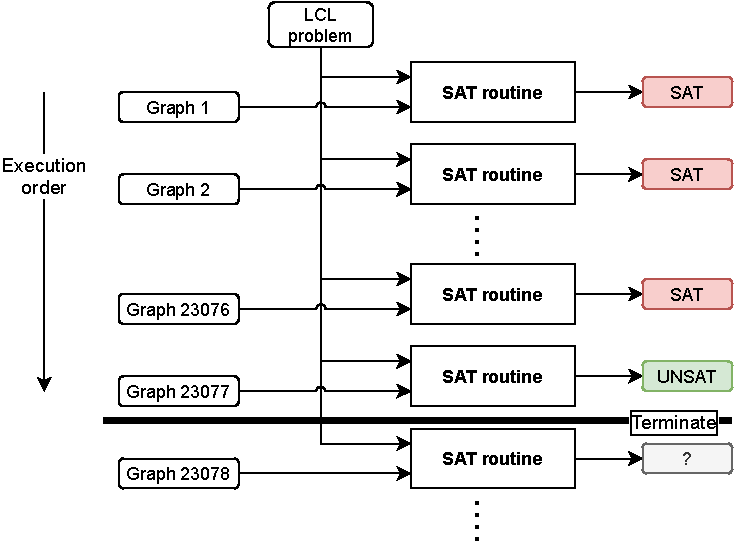
\includegraphics[]{diagrams/implementation_idea_diagram3.pdf}
\caption{An example of an execution of multiple SAT routines. Execution terminates at graph $23077$ when first UNSAT is encountered.}
\label{fig:implementatio:idea:2}
\end{figure}

%TODO biregular multigraphs?
%TODO LCL problems on biregular trees etc?

When we assume that an LCL problem $\Pi$ is solvable in PN, we mean that there exists a deterministic distributed algorithm $A$ in PN model, that finds a solution for all multigraphs i.e. algorithm $A$ works in every multigraph.
Every simple graph is also a multigraph, thus multigraphs are more relaxed in terms of definition.
Allowing parallel edges potentially gives us counter examples with smaller graph sizes when we use the increasing strategy i.e. our algorithm might terminate succesfully much earlier with the desired result and graphs do not necessarily become as complex as they would be with only simple graphs.
%TODO where to discuss about solutions that have been found only with multigraphs? Have we found any solutions with only simple graphs?
Smaller graphs mean less complexity and less performance required but as there are also more graphs to iterate, it is not so simple to justify allowing parallel edges only with this argument.
The main argument is that allowing parallel edges gives us more opportunities to find counterexamples.
It might be that in some problems we cannot even find counterexamples without parallel.

%This is indeed what we have used in this work.
%Probably, we have to iterate a lot of graphs.
%For this purpose we want to be able to generate the graphs.